\documentclass[ oneside,openright,titlepage,numbers=noenddot,headinclude,%1headlines,% letterpaper
                a4paper,
                footinclude=true,cleardoublepage=empty,abstractoff, % <--- obsolete, remove (todo)
                BCOR=5mm,paper=a4,fontsize=11pt,%11pt,a4paper,%
                british,%
                ]{scrreprt}

%********************************************************************
% Note: Make all your adjustments in here
%*******************************************************
\input{classicthesis-config}
\usepackage{setspace}
\usepackage[toc]{glossaries}
\makeglossaries


\newcommand{\Ebook}{E-book}
\newcommand{\ebook}{e-book}
\newcommand{\pdf}{\textsc{pdf}}
\newcommand{\epub}{\textsc{epub}}
\newcommand{\html}{\textsc{html}}
\newcommand{\xhtml}{\textsc{xhtml}}
\newcommand{\xml}{\textsc{xml}}
\newcommand{\css}{\textsc{css}}
\newcommand{\pdfdit}{\textsc{pdfdit}}
\newcommand{\troff}{\emph{troff}}
\newcommand{\Troff}{\emph{Troff}}
\newcommand{\ditroff}{\emph{ditroff}}
\newcommand{\Ditroff}{\emph{Ditroff}}
\newcommand{\COG}{\textsc{cog}}
\newcommand{\todo}[1]{\vspace{0.3in}\hspace{-1.5in}\textbf{\textcolor{red}{TODO:\hspace{0.5in}#1}}\vspace{0.3in}}
\newacronym[longplural=Frames per Second]{FPS}{fpsLabel}{Frame per Second}
%********************************************************************
% Hyphenation
%*******************************************************
%\hyphenation{put special hyphenation here}

% ********************************************************************
% GO!GO!GO! MOVE IT!
%*******************************************************

\includeonly{
% FrontBackmatter/Abstract,
% FrontBackmatter/Contents,
% Chapters/Chapter01,
% Chapters/Chapter02,
Chapters/Chapter03,
% Chapters/Chapter04,
% Chapters/Chapter05,
% Chapters/Chapter06,
% Chapters/Chapter07,
FrontBackmatter/Bibliography
}

\begin{document}
\frenchspacing
\raggedbottom
\selectlanguage{british} % american ngerman
%\renewcommand*{\bibname}{new name}
%\setbibpreamble{}
\pagenumbering{roman}
\pagestyle{plain}

%********************************************************************
% Frontmatter
%*******************************************************
\include{FrontBackmatter/DirtyTitlepage}

%*******************************************************
% Titlepage
%*******************************************************
\begin{titlepage}
	% if you want the titlepage to be centered, uncomment and fine-tune the line below (KOMA classes environment)
	\begin{addmargin}[-1cm]{-3cm}
    \begin{center}
        \large  

        \hfill

        \vfill

        \begingroup
            \color{Maroon}\spacedallcaps{\myTitle} \\ \bigskip
        \endgroup

        \myName \myOldDegree

        \vfill

         
        \spacedlowsmallcaps{Thesis submitted to \myUni} \\
        \spacedlowsmallcaps{for the degree of\ \myNewDegree} \\
        

        \spacedlowsmallcaps{\myTime}
        \vfill                      

    \end{center}  
  \end{addmargin}       
\end{titlepage}   
\include{FrontBackmatter/Titleback}

\cleardoublepage
%*******************************************************
% Dedication
%*******************************************************
\thispagestyle{empty}
%\phantomsection 
\refstepcounter{dummy}
\pdfbookmark[1]{Dedication}{Dedication}

\vspace*{3cm}

\begin{center}
    To myself
\end{center}

\medskip

\begin{center}
    My favourite of the 5 people\\who will ever read this\footnote{I will take the opportunity now to apologise for my poor sense of humour :)}
\end{center}
%\chapter{Foreword and Overview}
\setcounter{footnote}{-1}
This thesis is structured in a slightly unconventional manner:\footnote{but like all good computer scientists, we begin counting at zero\textsuperscript{$\star$}

 \vspace{0.8em}
\noindent \scriptsize{$\star$ except for the page numbering, because \LaTeX{} \emph{really} doesn't like having even numbers on right-facing pages\textsuperscript{$\dagger$}}

\vspace{0.8em} 
\noindent \tiny{$\dagger$ also the lack of a symbol for zero in Roman numerals rather spoils the joke}} its literature review is spread amongst the chapters, and sources are discussed within relevant areas of the text. Below is an outline of the thesis structure:

\vspace{1em}
\noindent Chapter~\ref{ch:intro} provides an overview of the present state of affairs of the electronic document world, with particular emphasis upon the technologies used in contemporary \ebook{} readers, and their benefits and drawbacks.

\vspace{1em}
\noindent Chapter~\ref{ch:malleable} takes a brief look at the history of movable type, and some of the techniques tradionally used in newspaper typesetting. Using some of these techniques as a basis, it then describes a novel paradigm for document representation that allows documents to fit a wide variety of screen sizes whilst maintaining high typographic quality. It then outlines a prototype implementation of a system to generate and display simple documents. Work in this chapter was published and presented at DocEng'11 in Mountain View, CA, USA.\hspace{0pt}\cite{Pinkney2011}

\vspace{1em}
\noindent Chapter~\ref{ch:floats} introduces a complete reimplementation of the system described in Chapter~\ref{ch:malleable} to enable its use on portable devices, and extends the devised model to include support for floating items such as figures and tables. Work in this chapter was published and presented at DocEng'13 in Florence, Italy.\hspace{0pt}\cite{Pinkney2013}

\vspace{1em}
\noindent Chapter~\ref{ch:bloat} addresses the issue of enlarged file sizes, and details various methods to keep file sizes to a minimum, where possible avoiding unnecessary increases computational complexity that would counter the work described in Chapters \ref{ch:malleable}~and~\ref{ch:floats}.

\vspace{1em}
\noindent Chapter~\ref{ch:analysis} provides technical and aesthetic analysis, focusing on the quantitative and qualitative aspects of the system as it runs at view-time, and includes the results of a user study of the system developed in the previous chapter.

\vspace{1em}
\noindent Finally, Chapter~\ref{ch:conclusions} evaluates the success of the project, and details areas of potential new research that have been encountered throughout the process.



\cleardoublepage
%*******************************************************
% Abstract
%*******************************************************
%\renewcommand{\abstractname}{Abstract}
\pdfbookmark[1]{Abstract}{Abstract}
\begingroup
\let\clearpage\relax
\let\cleardoublepage\relax
\let\cleardoublepage\relax

\chapter*{Abstract}
Computer document processing often starts with an abstract, structural, representation before entering a processing pipeline that creates a desired layout and appearance. Unfortunately the whole system resembles the successive irreversible stages of generating assembler code using a compiler. This `one-way function' behaviour is most obvious with \textsc{pdf}, which is tied to a completely fixed appearance once a document has passed through a one-way `trapdoor', such as Adobe Distiller. Any attempt to reflow a document that has been processed through one of these one-way functions, or to view it at some other size, is either frustrating or simply impossible, without regenerating the document from a more abstract, higher-level representation.

Other formats, for example \textsc{html}, do maintain enough semantic structure to allow documents to be rendered to fit any page size. Since document renderers for \textsc{html}-like documents must run on-the-fly, they tend to produce results that are typographically inferior to those of document renderers whose runtime complexity is not constrained by time.

The limitations of these two opposing paradigms have not been cause for concern until fairly recently. In a world of smart phones, \ebook{} readers, laptops, tablets, smart watches, internet-connected televisions, and of course not forgetting the humble printed page, it is no longer safe to assume that a document will be viewed only in one fixed presentation. Current fixed formats do not lend themselves to having their presentational properties partially unpicked and re-engineered, nor are current `flowable' formats capable of reliably producing acceptably typeset documents. This thesis details work towards defining a format that stores documents that can be `repurposed' to fit any arbitrary screen size on any device whilst maintaining high typographic quality, and without the the need for total reprocessing.

\endgroup

\vfill
%\cleardoublepage
%*******************************************************
% Publications
%*******************************************************
\pdfbookmark[1]{Publications}{publications}
\chapter*{Publications}
Some ideas and figures have appeared previously in \emph{Reflowable Documents Composed from
Pre-rendered Atomic Components}\cite{Pinkney2011}, published in the proceedings of the 2011
\textsc{acm} Symposium on Document Engineering.
\cleardoublepage
%*******************************************************
% Acknowledgments
%*******************************************************
\pdfbookmark[1]{Acknowledgments}{acknowledgments}

\begin{quote}{\slshape    
    In a badly designed book, the letters mill 
    and stand like starving horses in a field.
    In a book designed by rote, they sit 
    like stale bread and mutton on the page. 
    In a well-made book, where designer, compositor
    and printer have all done their jobs, 
    no matter how many thousands of lines and pages 
    they must occupy, the letters are alive. 
    They dance in their seats. 
    Sometimes they rise and dance in the margins and aisles. } \\ \medskip
    --- \defcitealias{Bringhurst2008}{Robert Bringhurst}\citetalias{Bringhurst2008} \citep{Bringhurst2008}
\end{quote}



\bigskip

\begingroup
\let\clearpage\relax
\let\cleardoublepage\relax
\let\cleardoublepage\relax
\chapter*{Acknowledgments}
Put your acknowledgments here.




\endgroup





\pagestyle{scrheadings}
\include{FrontBackmatter/Contents}
%********************************************************************
% Mainmatter
%*******************************************************
\pagenumbering{arabic}
% use \cleardoublepage here to avoid problems with pdfbookmark

\doublespacing
\cleardoublepage
\chapter{The rise of \ebook{}s} \label{ch:intro} % ``Introduction'' is too boring!

\marginpar{Note: this chapter is currently pretty much word for word the content of the interim
report. I'll update it when the rest is written.}

%\marginpar{Blurb re: portable devices, screen sizes etc}

The recent surge in popularity of devices such as the Amazon Kindle and the Apple iPad has vastly
increased the sale and distribution of \ebook{}s. Amazon.com recently announced\cite{Amazon.com2011}
that during the month of April 2011, Kindle Store sales outstripped print book sales by 105 to 100.
This figure does not include free \ebook{}s `sold' through the Kindle Store, which would skew the
figures significantly further. It was also reported that Amazon's UK Kindle Store, which opened in
September 2010, was, over the same period, outselling hardback books by a factor of two to one.
These ratios are likely to increase as time goes on.

\section{Devices}
\marginpar{Amazon\ed kindle apps for PC, iPhone, iPad, netbooks, \emph{actual} kindles\ldots a
plethora
of sizes! Many are battery powered. Don't want to kill the battery, but don't want output to look
crap.}
In addition to dedicated \ebook{} readers, such as the Amazon Kindle and the Sony Reader, many other
devices can be equipped to read the same \ebook{} files, such as tablets, mobile phones, laptops,
netbooks, and desktop PCs. Indeed, virtually every modern device with network connectivity and a
screen can be equipped to read \ebook{}s. Consequently, \ebook{} files are expected to be read on a
wide range of screen sizes and types.

\marginpar{something about range of screen sizes/types/pixel densities}

\section{File formats}
Three formats currently dominate the \ebook{} market: \epub{} and Mobipocket, which allow the
document to be formatted to fit the display device, and \pdf{}, which does not. Currently there is
no middle ground\ed a document may either be fully rendered to a fixed layout, or completely
unrendered, to be laid out at the mercy of a display device's decisions. Amazon's proprietary Kindle
format is derived from Mobipocket; \pdf{} and \epub{} are open standards.

\subsection{PDF}
\pdf{} was originally designed as a way of faithfully reproducing documents both on screen and in
print. For this reason, \pdf{} is almost entirely pre\-s\-en\-ta\-tion-oriented and will therefore
often include no information on the semantic structure of a given document. The archetypal \pdf{}
file will consist solely of drawing operators which describe the document pages. There is no
compulsion for these drawing operators to render the page in an order that might be considered
sensible: for example, if a \pdf{} generator program decided to render every character on a page in
alphabetical order, or radially outwards from the centre, the resulting file would still be
semantically valid, and the result might well be unnoticeable to the end user. This lack of imposed
semantic structure can make it difficult to infer the best way to `unpick' \pdf{} files to allow
their content to be reflowed into a new layout.

This is not to say that \pdf{} files \emph{cannot} represent the semantic stucture of their
content\ed indeed as early as 1999, \pdf{}~1.3 introduced \emph{logical structure}
facilities\cite{Adobe2001}, adding an optional \emph{structure tree} to the \pdf{} specification,
and \emph{tagged \pdf{}}, introduced in \pdf{}~1.4 in 2001, provides various extensions to this.
Unfortunately, \pdf{} documents which actually make good use of these facilities are few and far
between, even a decade after their introduction.

\marginpar{Mention why tagged \pdf{}/structure tree aren't particularly useful for reflow (ie helps
to unpick, but still need to re-typeset... no better off than html)}

\subsection{HTML based}
\label{html-format}
Both \epub{} and Mobipocket are largely based on \html{}. Whilst the use of \xml{}-like formats
allows the semantic structure of documents to be very well defined, in general their presentation
can only be specified in a very loose manner. The user is often presented with a choice of typefaces
and point sizes, allowing the reader software to render the document in essentially any arbitrary
way it chooses. Since an \html{}-derived format has no concrete presentation associated with it,
each time the document is displayed its layout must be recalculated, in a similar manner to the way
an interpreted programming language needs to be interpreted each time it runs. (We can therefore
compare \pdf{} to a compiled program: it is the result of an optimisation process performed upon
some semantically higher-level representation.) For an \ebook{} reader to maximise its battery life,
this `interpretation' needs to be as simple as possible, \ie{} the algorithm used must not be too
complex, since the more \textsc{cpu} cycles spent executing it, the
less time the \textsc{cpu} can spend idle, and thus the greater the drain on the battery.
Furthermore, the longer that is spent formatting the output, the longer the delay between page turns
on the device, and with the speed of \textsc{cpu}s used in these devices ($<$ 500 \textsc{MHz}) it
does not take too large an increase in computation for the page-turn time to become noticeable.



\section{Limitations}



The design paradigm of \pdf{}, conceived in the early 1990s\cite{Warnock1991}, was to form a perfect
analogue of the printed page, which would be exactly reproducible regardless of the system on which
the file was rendered. For this reason, it is possible to embed fonts within \pdf{} files, to ensure
faithful reproduction on any system, regardless of which fonts are actually installed. In general, a
well typset \pdf{} file looks good wherever it is displayed, but, stemming from the `digital sheet
of paper' paradigm, page sizes in a \pdf{} document are necessarily fixed at creation-time. An
overwhelming majority of \pdf{} documents are rendered for  US letter or A4 size paper. This is fine
if the document is to be printed and read. On a reasonably large screen, the document remains
perfectly readable; a 10'' netbook or tablet screen may provide acceptable reading. Anything much
smaller (notably mobile phones, and e-readers, such as the (non-DX) Kindle and the Sony Reader) and
a combination of zooming and panning is required 
in order to read the document. Documents may, of course, be rendered to a smaller page size, however
the problem still remains\ed it is unlikely that any one page size will be suited to \emph{all}
reading platforms. Most e-readers, using their native (i.e.\ non-\pdf{}) formats allow text to be
resized according to user preference. Indeed, it seems unnecessarily restrictive to force one size
of type upon the user. Of course, paper books suffer from this affliction; digital books need not.
Selling \ebook{}s separately in standard and large-print versions seems perverse when, for virtually
no difference in cost to the publisher/distributor, both can be included in one file. In fact,
storing the document at a higher, more abstract level than \pdf{} can allow the text to be rendered
at any desired size, but at the cost of the retention of high-quality typesetting afforded by
\pdf{}.

\marginpar{The rendering engines generally used in e-readers take a \emph{greedy} approach. That is,
they place as many words onto the current line as will fit, and then break, start a new line, and
repeat.}

\epub{} and Mobipocket, both based on \html{}, provide this necessary higher abstraction of
documents. This allows a font size to be specified, and the text to be rendered to closely fit the
screen. Line breaks and page breaks can then be calculated and inserted as necessary, in order to
wrap the text to fit the screen, and to paginate the content. The rendering engines used for
reflowable formats on e-reader devices are simplistic\ed but necessarily so. The battery life of
portable devices is lamentably low. Manufacturers of e-readers may claim their products have
batteries which can last for months, but this is principally due to the many shortcuts used when
laying out flowable content. As noted in section~\ref{html-format}, were these devices to use more
complex layout algorithms, which can produce far higher quality typeset output, it would soon emerge
than any savings made by using a low-power electronic paper screen would quickly disappear. In
addition to increasing battery usage, the higher computational complexity of these algorithms may
cause page turns to take longer, as each subsequent page is only rendered when a page turn is
requested. The time delay could be fixed reasonably easily by buffering between page turns, although
this does not solve the battery drain problem.



%\marginpar{Rendering engines are simplistic (but necessarily so, since need to save battery, and not
%take too long per page turn\ed although could buffer between page turns to avoid this) and thus
%don't produce nice results.}




\epub{} allows fonts to be embedded, but Mobipocket does not. Mobipocket files (and by extension,
Kindle files) are therefore restricted to be rendered in a typeface local to (and often chosen by)
the reader software. The Kindle, as an example, provides the user with a choice of `regular',
`condensed', or `sans-serif' for the main body text of its documents. There are bold and italic
variations of these, which are applied according to formatting instructions within the documents
themselves. Additionally, there is a typewriter-style font which document authors may choose to use
in the same manner. The Mobipocket specification supports a very limited subset of \html{} and
\css{}, which makes complex layouts, such as those involving arbitrary indentation or font size
changes, virtually impossible. Figures \ref{alices1} and \ref{alices2} demonstrate the well known
`Mouse's Tale' from Lewis Carroll's \emph{Alice in Wonderland}, in numerous formats.


\begin{figure}[tb]
\includegraphics[width=\textwidth]{gfx/alices1}
\caption[Document displayed in Calibre]{On the left is
an \epub{} version of Alice in Wonderland, displayed in Calibre (an open source desktop \ebook{}
viewer). On the right is the same file, converted to Mobipocket, also displayed in Calibre. Note
that in addition to the indentation being lost, the (embedded) font from the \epub{} is no longer
present in the Mobipocket file.}
\label{alices1}
\end{figure}

%\marginpar{Mobipocket\ed can't embed fonts... very limited choice of html to use. Reliant on
%rendering engine of device.
%\epub{}\ed can embed fonts, can style with \css{} pretty much arbitrarily, but still needs to be
%retypeset on each viewing and thus relies on the crappy built in rendering engine of the device.}

\epub{} is a little more flexible, in that it supports a more comprehensive range of \xhtml{} and
\css{}, and allows for arbitrarily complex styling. \epub{} files are still entirely reliant on the
rendering engine of the display device correctly displaying their content, as they have no concrete
layout associated with them.

\begin{figure}[tb]
\begin{center}
\vspace{-.3in}
\includegraphics[width=\textwidth]{gfx/alices2}
\end{center}
\vspace{-.3in}
\caption[The same document displayed on the Kindle]{On
the left is the Mobipocket version of Alice in Wonderland (from figure~\ref{alices1}) displayed on
the Kindle. Note that the sizing instructions appear to have been ignored. On the right is the free
version of Alice in Wonderland from the Kindle store, displayed on the Kindle. Note that no attempt
has been made to render the poem in a `tail' shape.}
\label{alices2}
\end{figure}

\section{``Good'' typesetting}
\label{goodtypesetting}
The paper \emph{Reflowable Documents Composed From Pre-rendered Atomic Components}\cite{Pinkney2011}
(attached as an appendix) goes into some detail, particularly in sections 2.1 and 2.2, of what sort
of properties to expect from good-quality typesetting.

Knuth and Plass's line breaking algorithm\cite{Knuth1981}, in conjunction with Liang's hyphenation
algorithm\cite{Liang1983}, breaks paragraphs into lines of text to fit a page, into what can be
considered to be an optimal configuration. \TeX 's default behaviour is then to alter the spacing
between words in order to justify the line to fit the measure of the page. More advanced methods
than simply stretching or shrinking the word spacing do exist, however. Robert Bringhurst, in
\emph{The Elements of Typographic Style}\cite{Bringhurst2008}, suggests that in addition to altering
word spacing, subtle changes to inter-character spacing and individual glyph widths (in the range of
$\pm$ 3\%) can produce more typographically and aesthetically pleasing results. This is discussed
further in section~\ref{edgecases}.

\marginpar{H+J. What is good H+J? Good hyphenation algorithm. Word spacing. Letter spacing. Glyph
reshaping. Must look at whole paragraph!}

\marginpar{Use of kerning. Use of ligatures where appropriate. Avoidance of widows/orphans.}



\chapter{The Malleable Document}\label{ch:malleable}  % ``Aims \& objectives''?? Booooring
%The real aim of this project is to produce documents that are adaptable to multiple viewing
apertures, but do not require total reprocessing to do so.

%\smarginpar{Malleable documents!}

\marginpar{Can we have one physical representation which fits to all devices \emph{and} is
efficient? Should we perform some pre-processing to the document to tailor it to a particular
device?}

Amazon's Kindle Store model provides a good example of the need for multipurpose documents\ed one
purchase may be viewed on any number of platforms\ed the desktop app, the mobile phone app, the
tablet app, and on the Kindle itself. Amazon does not currently provide any special dispensation for
any of the platforms it supports\ed every one receives the same source document to display.
Consequently, a Kindle book is effectively a jack of all trades, and master of none: instead of
looking good on any one platform, the books look mediocre on \emph{every} platform. The real
questions here are as follows:

\begin{itemize}
 \item Is it possible to have one physical representation which typesets well on \emph{all}
platforms whilst remaining efficient enough not to cause excessive battery drain?
 \item Is it possible to identify invariant features common to many renderings to reduce the need
for processing on the display device?
 \item Should a more abstract, higher level of document be provided from which lower-level
device-specific derivatives can be produced?
\end{itemize}
  
The desire is to develop some document format which is neither as `solid' as a PDF nor as `liquid'
as HTML, but somewhere in between (perhaps termed a \emph{malleable document}). Something which is
mostly formed, but can be gently massaged to fit the display as necessary.



\cleardoublepage
\chapter{Floatable Blocks}\label{ch:floats}

% Required implementation:
% \begin{itemize}
%     \item extension of chapter 2 code to support floats
%     \item tradeoffs between Plass\cite{Plass1981} pagination and `dumb' pagination. Should floats be
%     `floatable'?
%     \begin{itemize}
%         \item how floatable?
%         \item how much effort do we put in before it stops being worth it?
%     \end{itemize}
%     \item Floats across multiple columns?
%     \begin{itemize}
%         \item simple multiples of galley width/line height
%     \end{itemize}
%     \item Bringhurst's suggestion\cite{Bringhurst2008} of making blocks take up multiples of the
%     leading to always keep text in phase (could even factor this into chapter 2 implementation)
% 
% \end{itemize}

The system described in Chapter~\ref{ch:malleable} supports only simple documents that are composed solely from text. Many (perhaps most) real-world documents contain figures, diagrams, illustrations, tables etc., so consideration must be given towards how these should be handled.
This chapter extends the work of the previous chapter to allow floatable graphical blocks, whose absolute position within a document's text may vary, depending upon the layout.

\section{Implementation}

The implementation of the system described in the previous chapter is deeply rooted within \pdf{}, and requires the custom-written plugin (see Section~\ref{sec:acroplugin}) for Adobe Acrobat to view the documents. Consequently, it is difficult to test that particular implementation on any device which is not running Microsoft Windows and does not have a fully licensed version of Adobe Acrobat. Effectively, this rules out any mobile \ebook{} readers.

Almost all \ebook{} readers support the \epub{} format,\marginpar{Amazon's Kindle is one of the few devices that does \emph{not} support \epub{}} which is principally built upon \html{}, \css{}, and JavaScript. With this in mind, it was decided to reimplement the system using these technologies, in order that it might be tested on \ebook{} hardware. 



\subsection{Document Generation}
\label{sec:docgen}




In the system described in the previous chapter, the generation of malleable documents was a rather labour-intensive process, involving running the source document through \troff{} and \pdfdit{}. In the case of documents with galleys of more than one width, modifications needed to be made, by hand, to the document structure tree of the resultant \pdf{} files.

Adding or removing characters to the source of a \pdf{} file is no trivial matter, since the \textsc{xref} table, which stores the byte offsets of all \glspl{COSObject} within the file, is no longer correct. (Acrobat does kindly offer to fix this problem if it detects it, but it has the side effect of discarding any data it does not recognise. Clearly losing the document structure tree is undesirable.) The \textsc{xref} table can either be fixed programatically, or by a painstaking process involving a hex editor and a lot of patience. Significant lack of patience meant that there was only ever one multiple galley-width test document produced for the previous system.

Since the new system no longer relies on \COG{}-\pdf{}, the reliance on \troff{} and \pdfdit{} is also abated. Consequently, a sensible approach is to produce a completely bespoke typesetting tool, allowing unneeded features to be removed, and some finer-grained controls (for example the line-breaking and hyphenation algorithms) to be added.



In the new system, the source document is described in terms of separate logical blocks; a block is either designated as a `float', or as a `paragraph'. Floats are currently limited to only referencing images (with an optional size parameter). Paragraphs, on the other hand, are described by their desired textual content. This is deliberately simplistic. It is envisaged that in a real system, the source document would have a richer language, perhaps marked up in a form similar to \LaTeX{} source, or in \xml{}.

Next, the source document is passed through a program to produce the output that becomes the malleable document itself. This program passes the text of each paragraph through a line breaking algorithm (for example an implementation of the Knuth-Plass algorithm). Each paragraph is rendered multiple times, once for each galley width, in order to produce the document's multiple galley renderings. Each line of each rendering of each paragraph is converted into a list of its composite words. Each of these words has an associated offset (in points) from the start of the line, which is later used when drawing the text.

The content of the floats is largely left unchanged. A reference to the image, along with its required dimensions, is simply passed through to the output. If dimensions were not explicitly specified in the source document, the pixel size of the image itself is used.

Finally, once the whole of the source document has been processed, the rendered content is output\,---\,in the form of the document structure tree shown in figure~\ref{fig:tree}\,---as a multi-dimensional JavaScript array. This becomes the data representing the source document, which, in conjunction with the viewer defined in the next section, becomes a \emph{malleable document}.




\subsection{The Viewer}
\label{sec:viewer}

In order to circumvent the browser's default text layout algorithm, and to ensure that our ``high quality'' pre-computed text layout is used, the viewer must specify the absolute position of every word on each line, in a manner not dissimilar to the internals of a PDF file. The document generator described in the previous section ensures that all the information needed to lay out the text is contained within the generated JavaScript array representing the document structure tree.

% The JavaScript array representing the document structure tree, output by the process described in the section above, contains all the information needed to lay out the text in the manner defined by whichever line breaking algorithm was used.  

When the viewer is launched, it decides which is the most appropriate galley rendering to display, based on some metric of which rendering will be most aesthetically pleasing. Since it appears to work well, the metric defined in Chapter~\ref{ch:malleable} is used, which attempts to balance a penalty for excessive inter-column whitespace against a penalty for too many columns. 


\subsubsection{Floats with a Queue}
The first attempt at supporting floats took inspiration from \LaTeX, which places floats into a queue until it finds somewhere it deems appropriate to place the first float. In order to emulate this, two queues were defined: the \emph{float queue}, and the \emph{line queue}. (`Line queue' is perhaps a slight misnomer, but it is somewhat snappier than `non-floating items queue'.)


If both queues are empty, as they will be at the start of the layout process, the document structure tree is traversed, and when the first paragraph-level item (see figure~\ref{fig:tree}) is encountered, its subcomponents (of the chosen galley rendering) are added to the requisite queue: lines to the line queue, and floats to the float queue.

Once at least one of the queues is not empty, the document begins to be laid out. If the float queue is nonempty, and the first float in the queue will fit below the last typeset item, is is placed on the page. If not, items from the line queue are placed one by one, until no more will fit in the current column. When this happens, a new column is started, and the first float in the float queue is output. Whenever the line queue is depleted, and no floats in the float queue will fit at the current point on the page, the next paragraph-level item from the document structure tree is queued. This process is illustrated in Figure~\ref{fig:float-flowchart}.

\begin{figure}
  \begin{center}
  \includegraphics[height=\textheight]{gfx/floatqueueflowchart}
  \end{center}
  \caption{Flowchart describing the two-queue float algorithm}
  \label{fig:float-flowchart}
\end{figure}


Whilst this approach does produce reasonable layouts, and handles floats well without the need for backtracking, it is not particularly conducive to producing layouts with floats that span multiple columns. The queue-based layout described above is fairly dumb: although it knows about the size of each component that it lays out, it does not remember the history of the positions of any of the components it has already laid out. This makes it difficult to have items that span more than one column, because there is no mechanism to mark space on the page as being reserved. In order to do this, another approach must be taken.

\subsubsection{A Grid-Based Layout}
% - Support of floats
    % - Queue system
    % - Grid/array system (no need for queue)
    % - Multicolumn floats
        % - issues with spanning \& pagination
A simple method for allowing parts of a page to be reserved is to break it up into a grid. Many newspapers use a grid-based layout (an example is shown in figure \ref{fig:gridlayout}). Following the example set by these newspapers, the grid is defined to have a row height of the leading the document's body text, with one column in the grid per column of text.

\begin{figure}
    \includegraphics[width=\textwidth]{gfx/newspaper-cropped}
    \caption[An example of a grid-based layout]{An example of a grid-based layout in a UK newspaper. Note how all the baselines of the main body text are aligned to a common grid, and that all items span integer multiples of columns.}
    \label{fig:gridlayout}
\end{figure}

The viewer uses the dimensions of the float, as specified in the document structure tree (see section \ref{sec:docgen}), to determine how many columns it should span. The float is scaled to span the integer multiple of column widths that most closely matches its `natural' size, though for reasons that should hopefully be obvious, this number is limited to a minimum of 1, and a maximum of the number of columns on the page. Additionally, checks are made to ensure that the scaling will not cause height of the figure to exceed that of the page.

An advantage of this grid-based approach is that it no longer requires the use of queues, either for lines, or for floats. The viewer simply traverses the document structure tree, placing each item in the first available place in the grid. In the case of floats, or other items larger than multiples of the main leading, spaces in the grid can be marked as reserved, to prevent other items from trampling over their reserved space. If a float will not fit directly below the previous item to be placed, the grid is walked over until a sufficiently sized gap can be found. Figure~\ref{fig:screengrab} shows an example of a document laid out with our system.

\todo{Discuss pagination in detail and issues that pagination introduces for multi-column spans}

\begin{figure}
    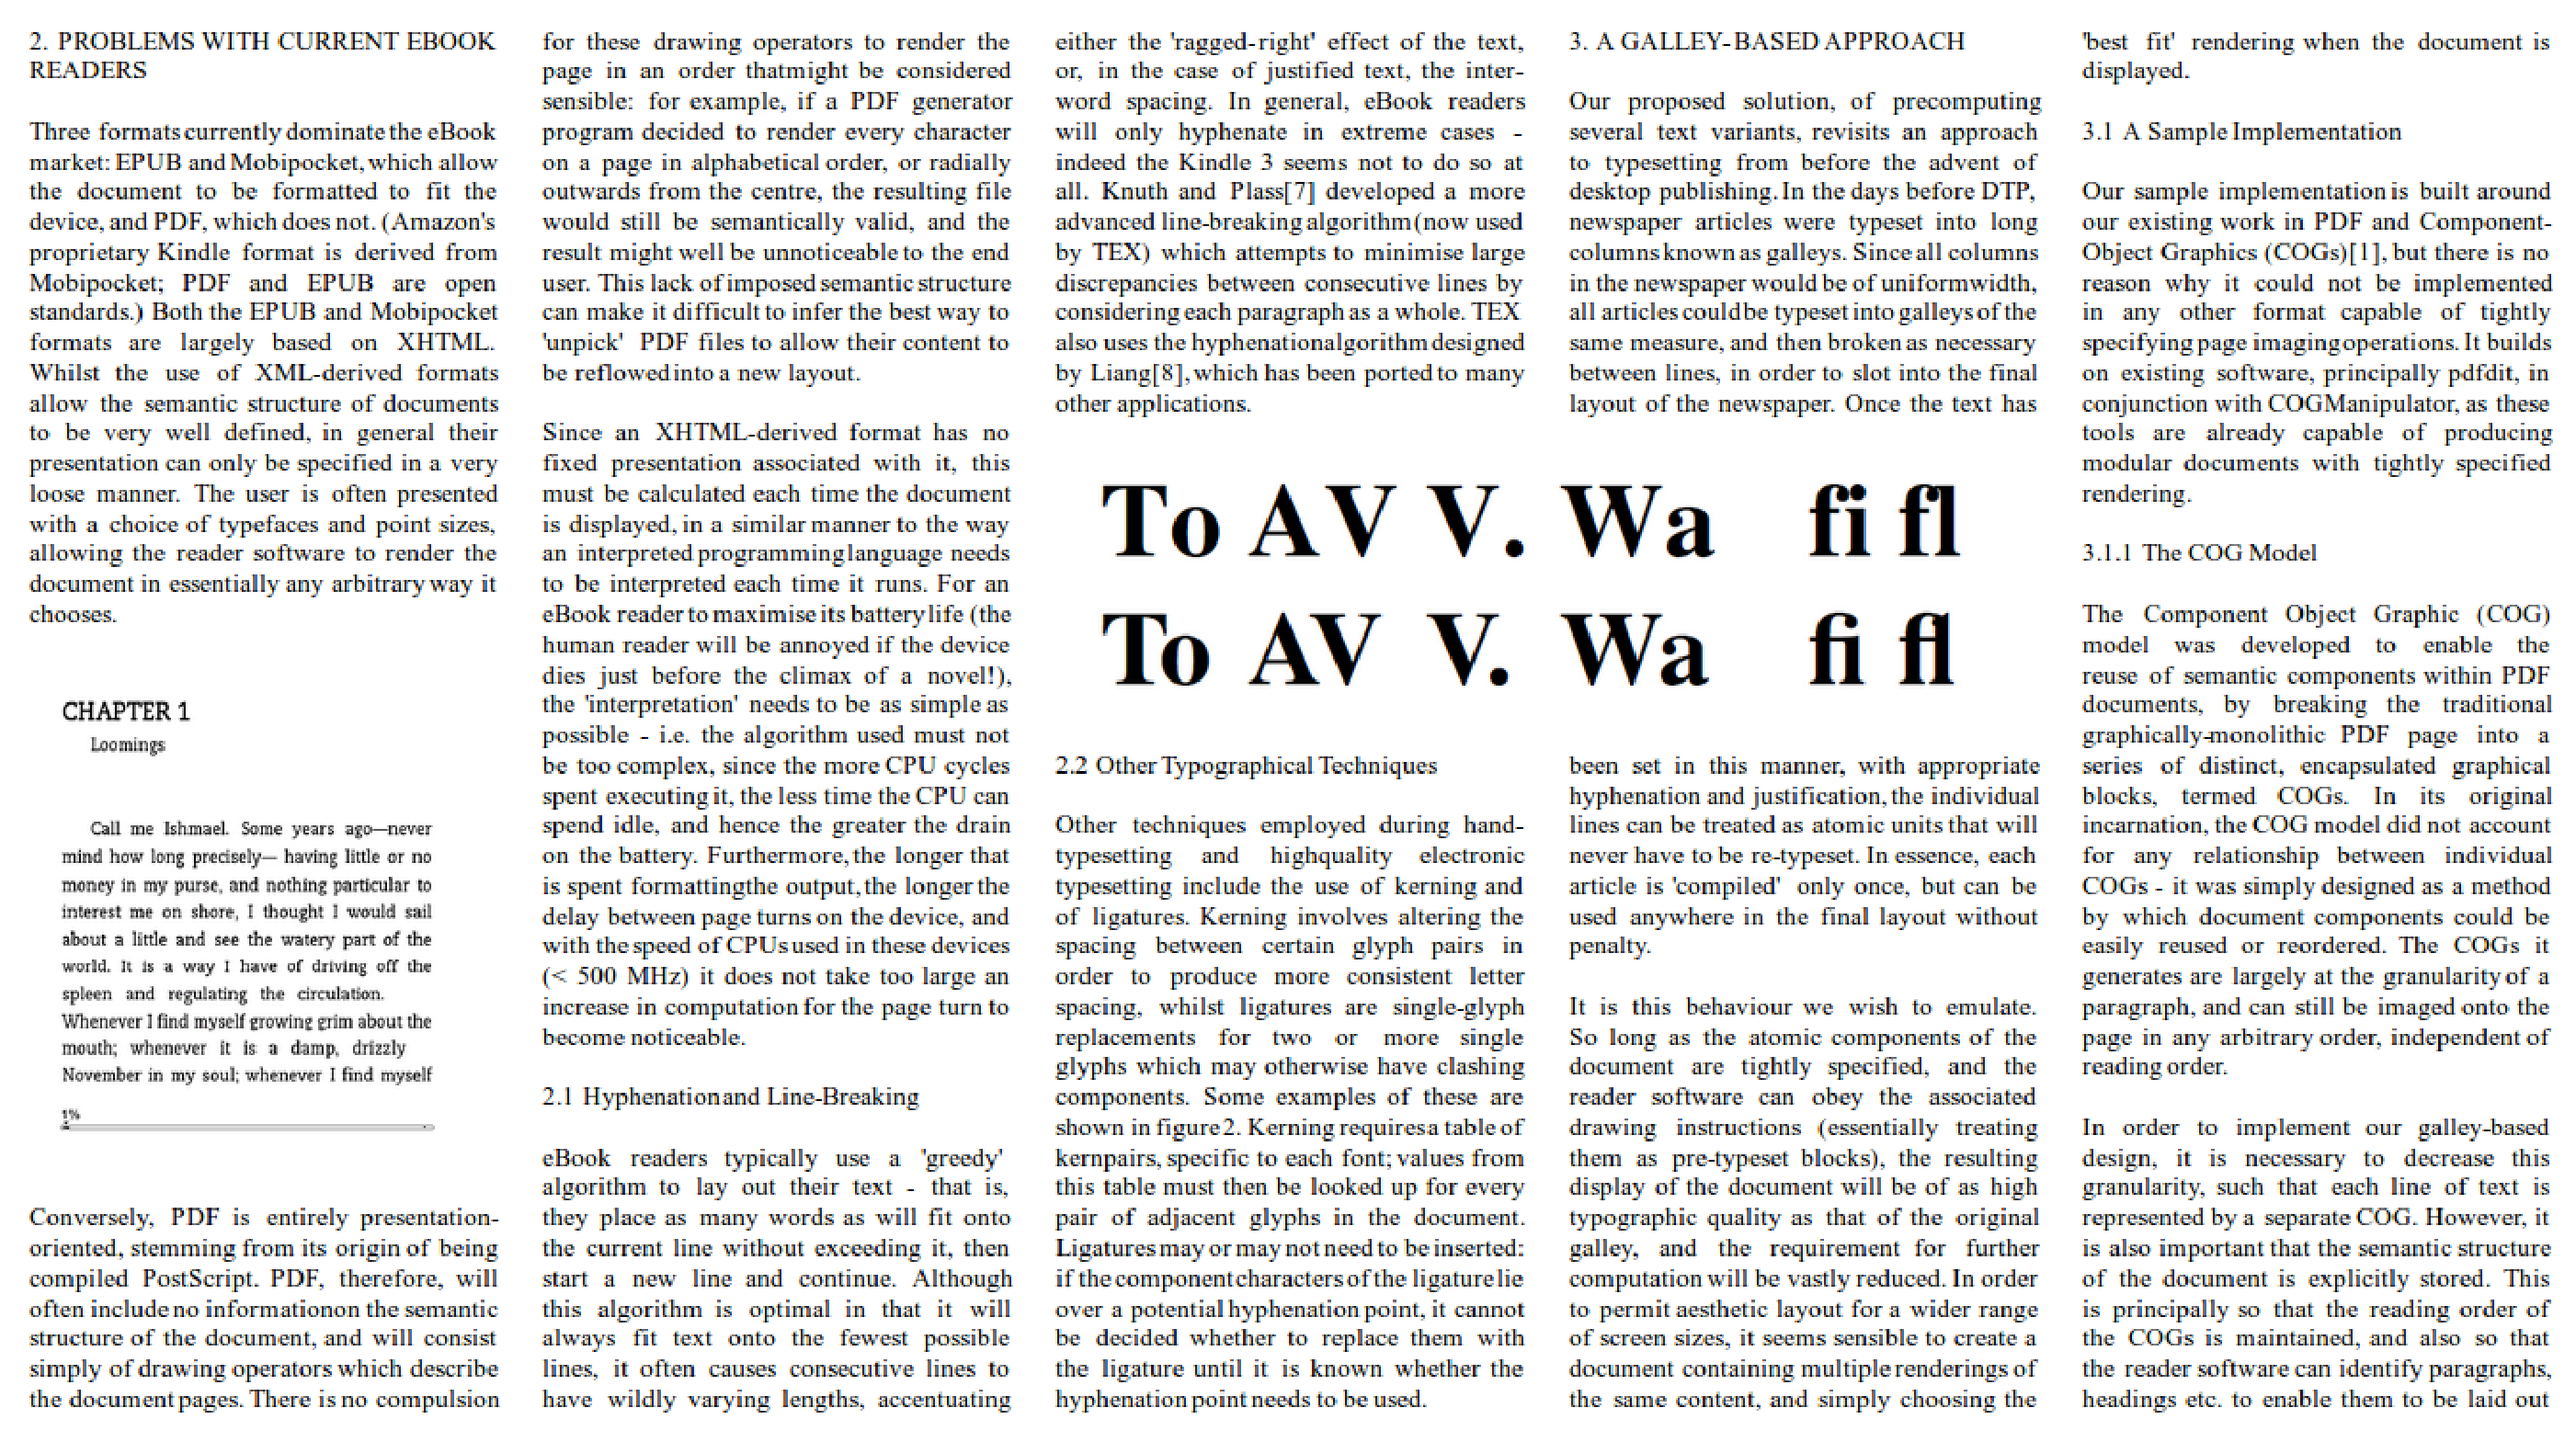
\includegraphics[width=\textwidth]{gfx/floatrendering}
    \caption[A sample rendering with multi-column floats]{An excerpt from \cite{Pinkney2011}, typeset and rendered by our new system.}
    \label{fig:screengrab}
\end{figure}

The system also supports point size changes. Although every galley is rendered in the same point size, at view time this can be scaled up or down, based on the preference of the user. The gaps between words are scaled proportionally, to allow the text to remain correctly justified.


%%%%%%%%%%%%%%%%%%%%%%%%%%%%%%%%%%%%%%%%%%%%%%%%%%


\section{Performance}
\label{sec:performance}

\subsection{Computational}
The layout system described herein works in a similar manner to a first-fit line-breaking algorithm, in that it places elements on the page in order, in the first place they will fit. Items that are the same size as a single grid cell, such as lines of text set in the main point size, can simply be placed in the first empty slot in the current column, or the first empty slot in the next column, should there be no empty spaces.  For the placement of items that are larger than a single grid cell, there is some overhead required to step through the grid until a suitable position can be found. Once a position has been found, each grid cell that it overlaps must be marked as being reserved.

Whilst this algorithm does have a greater-than-linear time complexity, the problem size is actually reduced in comparison to a first-fit text layout algorithm, since the system uses lines of text as its atomic units, rather than individual words. For this reason, it is felt that this algorithm should still be efficient enough to merit its use on portable \ebook{} readers.


    % - algorithm analysis?\\
    % - some physical timings?

\subsection{Aesthetic}
Aesthetically speaking, our system produces layouts that we feel most people would consider to be `good'. The system can guarantee use of a high-quality line breaking algorithm, since it has effectively been compiled in, and so the only remaining concern is that the columns of text and floats are laid out in a pleasing manner.

Harrington et al.~\cite{Harrington2004} identified nine aesthetic measures for automated document layout. A number of these measures (alignment, regularity, uniform separation, white-space free-flow, uniformity) are particularly well satisfied by our system, due to its use of a grid to provide regular layout.

\todo{Include picture of Greeked text that Steve printed out\ed{}mine vs web browser}
%   - Greeking\\
%       - Default browser layout vs mine\\
%       - Look at \cite{Harrington2004} for some measures and say why mine is awesome\\
%   - some discussion of choices of galley widths for best performance
    

%%%%%%%%%%%%%%%%%%%%%%%%%%%%%%%%%%%%%%%%%%%%%%%%%%



\section{Extensions}
\label{sec:future}
The system described in this chapter has only very basic support for floats. A particular limitation is that unlike paragraphs, each float has only one rendering, which must be scaled up or down as required, to fit across multiples of columns. Whilst for image-based figures or illustrations, this is probably already the desired behaviour, other types of floats, such as tables or code listings, would almost certainly benefit from the inclusion of multiple width renderings, with the choice of which rendering to display to be made at view-time. % Say that these could be differing hand-renderings, or automated from some source? Probably don't need to...

% coordinating breakpoints? might leave this until I have something sensible to say

Since the malleable document and viewer are composed entirely from HTML, CSS, and JavaScript\,---\,the core technologies behind EPUB\,---\,modifying the system to produce self-contained EPUB files seems an obvious next step.

%%%%%%%%%%%%%%%%%%%%%%%%%%%%%%%%%%%%%%%%%%%%%%%%%%

\chapter{Dealing with File Bloat}\label{ch:bloat}
\redmarginpar{Have done the groundwork for this chapter (results in table~\ref{tab:filesize}) but need to do some more on comparing different compression schemes, and then write about it.}

\section{Rationale}
In the system thus far described in this thesis, the emphasis has been firmly upon reducing the computational complexity of layout operations at view-time of a document, and therefore little consideration has been given to the filesize of the resultant malleable documents.

\todo{Put in some pdfdump output comparing ``normal'' pdfs with my malleable ones (maybe as an appendix)}

The resultant tradeoff between filesize and required computation has previously been justified on the basis that storage is both cheap (as of 2013 one US dollar will buy around two gigabytes of \textsc{nand} flash memory) and light; and batteries, although not enormously expensive either, already comprise a significant proportion of the overall mass of most portable devices suitable for reading \ebook{}s. The upshot is that adding more storage to a device has little impact upon devices' aesthetics, but that adding extra battery life (emerging nanotube battery technology notwithstanding) would result in vast increases in the devices' overall bulk and mass.

Despite this, it seems perverse to make no attempt at all to keep filesizes as small as possible, as long as there are no (or limited) impacts upon the required computation at view-time.

\section{Implementation}
The most obvious saving that can be made is with the duplication of a document's textual content. The systems described in chapters \ref{ch:malleable}~and~\ref{ch:floats} both contain as many copies of the document text as there are pre-rendered galleys; in practice, though, there is no real need for more than one copy to be present in the file. Two approaches to this problem were considered.

\subsection{Pointers into the Source Text}
The first approach to be considered was to include the source text of the document in its entirety, and for each rendering to contain only pointers to the relevant sections of text, instead of the words themselves. These pointers can either be physical\redmarginpar{I don't think ``physical'' is the right word here. What is???} (in the form of a character offset from the start of the text) or logical (in the form \emph{paragraph m, word n}). If the document text is to be included as a plaintext string, physical pointers are easier to use than logical: logical pointers either require an auxiliary data structure to map the logical pointers to physical ones, or for the document text to be stored in a format reflecting the logical structure, \ie{} not in plain text.

A drawback of using this approach is that on occasion, the output of the linebreaking process does not exactly match the input: for example in the case where words are hyphenated (requiring one word to be broken into two parts, and the addition of a hyphen) or where certain glyphs may be substituted for others (such as with the use of ligatures, where a glyph pair or triplet may be replaced with a single glyph).



\subsection{Use of a Dictionary}
The second approach considered was the use of a \emph{dictionary} (or \emph{map}) to act as a lookup table for each word-level item produced by the linebreaking process.

\begin{figure}
  \begin{center}
  \includegraphics[width=\textwidth]{gfx/wordfreq}
  \end{center}
  \caption[Word frequencies in various documents]{Word frequencies in various documents, plotted on a log-log scale. All of these documents, despite their varying lengths, appear to conform well with Zipf's Law. }
  \label{fig:wordfreq}
\end{figure}

If, for example, if the word ``shall'' appears several times in a document (in the King James Version of the Bible it appears 9760 times, and in the complete works of Shakespeare 3016 times) it is only stored once in the dictionary. As long as a word's key is lexicographically shorter than the word itself, it can be guaranteed that some redundancy has been removed from the data.


\section{Results}

\subsection{Ordered dictionary with absolute positioning}

\begin{figure}
  \begin{center}
  \includegraphics[width=\textwidth]{gfx/scaling}
  \end{center}
  \caption[Filesize versus number of renderings, using absolute positioning]{Filesize in bytes, for a selection of documents that contain varying numbers of galley renderings, using an ordered dictionary and absolute positioning}
  \label{fig:sizescale}
\end{figure}

\begin{figure}
  \begin{center}
  \includegraphics[width=\textwidth]{gfx/scalingpersrc}
  \end{center}
  \caption[Filesize as a proportion of source document size, versus number of renderings, using absolute positioning]{Filesize as a proportion of source document filesize, for a selection of documents that contain varying numbers of galley renderings, using an ordered dictionary and absolute positioning}
  \label{fig:sizescalepersrc}
\end{figure}

\begin{figure}
  \begin{center}
  \includegraphics[width=\textwidth]{gfx/scalingpersrcpern}
  \end{center}
  \caption[Filesize as a proportion of source document size, per rendering, versus number of renderings, using absolute positioning]{Filesize as a proportion of source document filesize and per galley rendering, for a selection of documents that contain varying numbers of galley renderings, using an ordered dictionary and absolute positioning}
  \label{fig:sizescalepersrcpern}
\end{figure}


\subsection{Ordered dictionary with relative positioning}

\begin{figure}
  \begin{center}
  \includegraphics[width=\textwidth]{gfx/scalingdeltas}
  \end{center}
  \caption[Filesize versus number of renderings, using relative positioning]{Filesize in bytes, for a selection of documents that contain varying numbers of galley renderings, using an ordered dictionary and relative positioning, with word widths stored in the dictionary}
  \label{fig:sizescaledeltas}
\end{figure}

\begin{figure}
  \begin{center}
  \includegraphics[width=\textwidth]{gfx/scalingdeltaspersrc}
  \end{center}
  \caption[Filesize as a proportion of source document size, versus number of renderings, using relative positioning]{Filesize as a proportion of source document filesize, for a selection of documents that contain varying numbers of galley renderings, using an ordered dictionary and relative positioning, with word widths stored in the dictionary}
  \label{fig:sizescaledeltaspersrc}
\end{figure}

\begin{figure}
  \begin{center}
  \includegraphics[width=\textwidth]{gfx/scalingdeltaspersrcpern}
  \end{center}
  \caption[Filesize as a proportion of source document size, per rendering, versus number of renderings, using relative positioning]{Filesize as a proportion of source document filesize and per galley rendering, for a selection of documents that contain varying numbers of galley renderings, using an ordered dictionary and relative positioning, with word widths stored in the dictionary}
  \label{fig:sizescaledeltaspersrcpern}
\end{figure}

\begin{table}
    \myfloatalign
  \begin{tabularx}{\textwidth}{lXXXXXX} %\toprule
    & \multicolumn{2}{l}{\textsc{source text}} & \multicolumn{2}{l}{\textsc{orig. scheme}} & \multicolumn{2}{l}{\textsc{dictionary}} \\
    & \textsc{plain} & \textsc{gz} & \textsc{plain} & \textsc{gz} & \textsc{plain} & \textsc{gz} \\ \midrule
    PBB11~\cite{Pinkney2011} & 23\textsc{k} & 9.4\textsc{k} & 627\textsc{k} & 145\textsc{k} & 314\textsc{k} & 111\textsc{k} \\ \midrule
    King James Bible & 4.3\textsc{m} & 1.4\textsc{m} & 144\textsc{m} & 32\textsc{m} & 73\textsc{m} & 24\textsc{m} \\ 
    \bottomrule
  \end{tabularx}
  \caption[Comparison of filesizes]{Comparison of filesizes using various encoding methods}  \label{tab:filesize}
\end{table}
\chapter{Technical Analysis}\label{ch:techanalysis}



\chapter{Performance and Evaluation}\label{ch:eval}



\chapter{Conclusions, Evaluation, and Future Work}\label{ch:conclusions}



\singlespacing

% ********************************************************************
% Backmatter
%*******************************************************
\appendix
\cleardoublepage
%\part{Appendix}

%%********************************************************************
% Appendix
%*******************************************************
% If problems with the headers: get headings in appendix etc. right
%\markboth{\spacedlowsmallcaps{Appendix}}{\spacedlowsmallcaps{Appendix}}
\chapter{Source Code Listings}


\section{Java Paragraph Splitter}
\label{app:parsplitter}
\subsection{ParSplitter.java}
\lstinputlisting[nolol,language=Java,tabsize=4,stringstyle=\color{blue},basicstyle=\ttfamily\scriptsize]{../../../../public_html/JSReflow/ParSplitter/src/ParSplitter.java}

\newpage

\section{C Linebreaker}
\label{app:linebreaker}
\subsection{main.c}
\lstinputlisting[nolol,language=c,tabsize=4,stringstyle=\color{blue},basicstyle=\ttfamily\scriptsize]{../../../../public_html/JSReflow/LineBreak/main.c}

\newpage

\subsection{Formatter.h}
\lstinputlisting[nolol,language=c,tabsize=4,stringstyle=\color{blue},basicstyle=\ttfamily\scriptsize]{../../../../public_html/JSReflow/LineBreak/Formatter.h}

\newpage

\subsection{Formatter.c}
\lstinputlisting[nolol,language=c,tabsize=4,stringstyle=\color{blue},basicstyle=\ttfamily\scriptsize]{../../../../public_html/JSReflow/LineBreak/Formatter.c}

\newpage

\subsection{parseAFM.h}
\emph{Used to parse the AFM (Adobe Font Metrics) files to give the typesetter the required knowledge of the typeface.}
\lstinputlisting[nolol,language=c,tabsize=4,stringstyle=\color{blue},basicstyle=\ttfamily\scriptsize]{../../../../public_html/JSReflow/LineBreak/parseAFM.h}

\newpage

\subsection{parseAFM.c}
\emph{Used to parse the AFM (Adobe Font Metrics) files to give the typesetter the required knowledge of the typeface.}
\lstinputlisting[nolol,language=c,tabsize=4,stringstyle=\color{blue},basicstyle=\ttfamily\scriptsize]{../../../../public_html/JSReflow/LineBreak/parseAFM.c}

\newpage

\cleardoublepage
\chapter{A Sample Malleable Document}
\label{app:sampledoc}
\section{butterley.html}
\emph{the \textsc{html} page within which the document is displayed}
\lstinputlisting[nolol,language=html,tabsize=4,stringstyle=\color{blue},basicstyle=\ttfamily\scriptsize]{../../../../public_html/JSReflow/butterley.html}

\section{style.css}
\emph{generic formatting instructions for the document}
\lstinputlisting[nolol,tabsize=4,stringstyle=\color{blue},basicstyle=\ttfamily\scriptsize]{../../../../public_html/JSReflow/styles.css}
\newpage

\section{script-json.js}
\emph{the script used to perform the layout at view-time}
\lstinputlisting[nolol,language=c,tabsize=4,stringstyle=\color{blue},basicstyle=\ttfamily\scriptsize]{../../../../public_html/JSReflow/script-json.js}

\newpage

\section{butterley.js}
\emph{the layout data of the document itself}
\lstinputlisting[nolol,language=c,tabsize=4,stringstyle=\color{blue},basicstyle=\ttfamily\scriptsize]{../../../../public_html/JSReflow/butterley.js}

%********************************************************************
% Other Stuff in the Back
%*******************************************************
\include{FrontBackmatter/Bibliography}
\include{FrontBackmatter/Colophon}
\include{FrontBackmatter/Declaration}
% ********************************************************************
% Game Over: Restore, Restart, or Quit?
%*******************************************************
\end{document}
% ********************************************************************


% **************************************************************************************************************
% A Classic Thesis Style
% An Homage to The Elements of Typographic Style
%
% Copyright (C) 2011 Andr\'e Miede http://www.miede.de
%
% If you like the style then I would appreciate a postcard. My address 
% can be found in the file ClassicThesis.pdf. A collection of the 
% postcards I received so far is available online at 
% http://postcards.miede.de
%
% License:
% This program is free software; you can redistribute it and/or modify
% it under the terms of the GNU General Public License as published by
% the Free Software Foundation; either version 2 of the License, or
% (at your option) any later version.
%
% This program is distributed in the hope that it will be useful,
% but WITHOUT ANY WARRANTY; without even the implied warranty of
% MERCHANTABILITY or FITNESS FOR A PARTICULAR PURPOSE.  See the
% GNU General Public License for more details.
%
% You should have received a copy of the GNU General Public License
% along with this program; see the file COPYING.  If not, write to
% the Free Software Foundation, Inc., 59 Temple Place - Suite 330,
% Boston, MA 02111-1307, USA.
%
% **************************************************************************************************************
% Note:
%    * You must not use "u etc. in strings/commands that will be spaced out (use \"u or real umlauts instead)
%    * New enumeration (small caps): \begin{aenumerate} \end{aenumerate}
%    * For margin notes: \marginpar or \graffito{}
%    * Do not use bold fonts in this style, it is designed around them
%    * Use tables as in the examples
%    * See classicthesis-preamble.sty for useful commands
% **************************************************************************************************************
% To Do:
%		 * [high] Check this out: http://www.golatex.de/koma-script-warnung-in-verbindung-mit-listings-package-t2058.html
%    * [medium] mathbb in section-titles/chapter-titles => disappears somehow in headlines!!!
% **************************************************************************************************************